\documentclass[tikz, border=5mm]{standalone}
% \usepackage[utf8]{inputenc}

% Librerías necesarias para geometrías y posicionamiento relativo
\usetikzlibrary{shapes.geometric, arrows.meta, positioning, fit, backgrounds}

\begin{document}

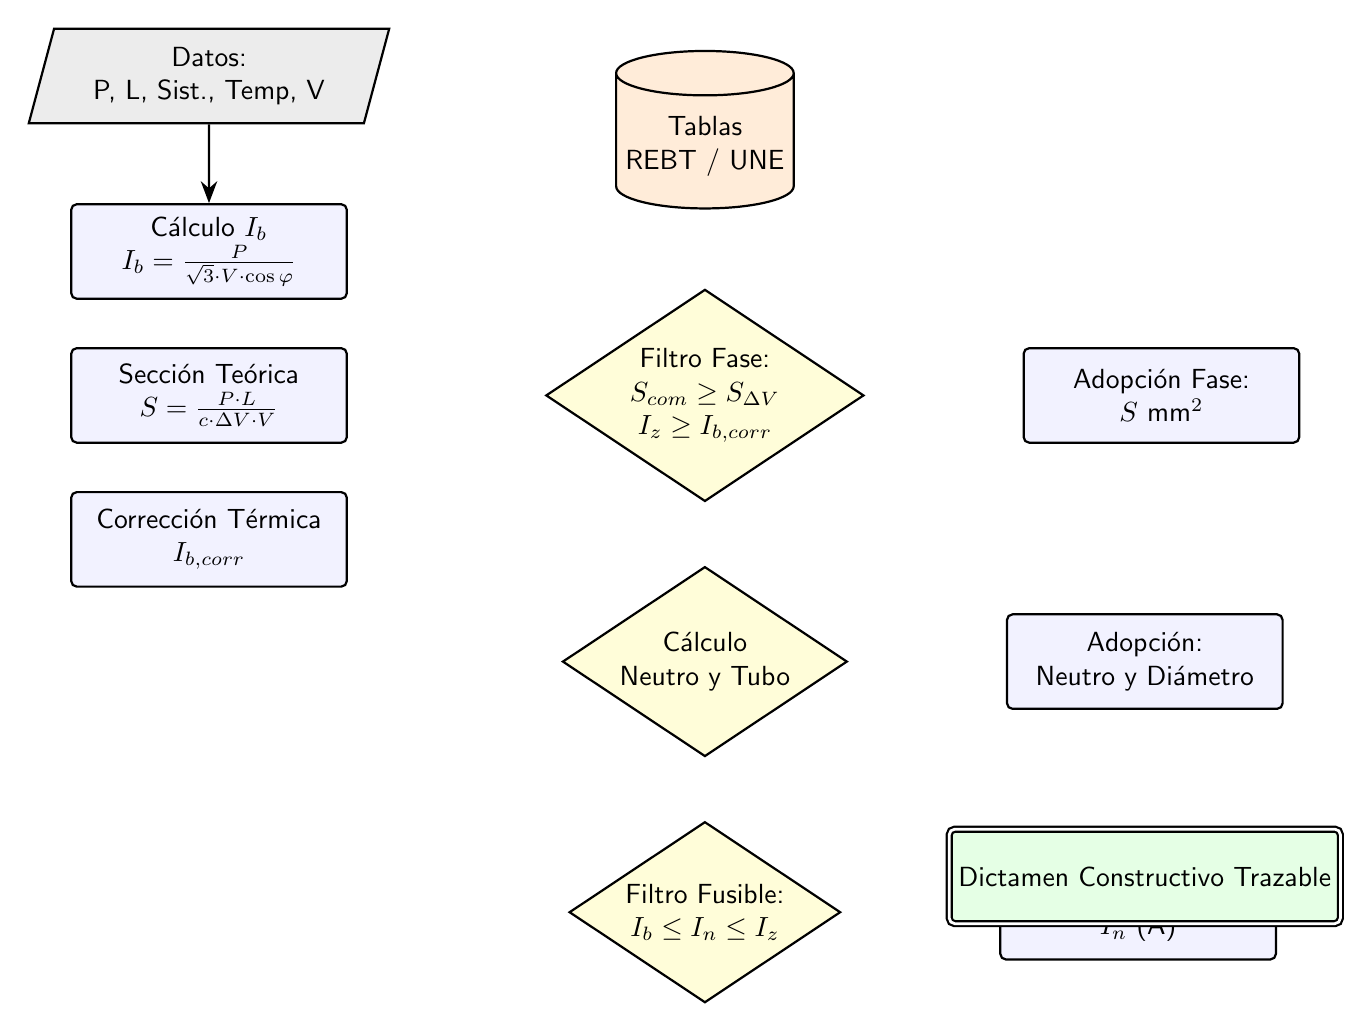
\begin{tikzpicture}[
    % Definición global de estilos de nodos
    base/.style = {draw=black, thick, minimum height=1.2cm, align=center, font=\sffamily},
    input/.style = {base, trapezium, trapezium left angle=75, trapezium right angle=105, fill=gray!15, minimum width=3.5cm},
    process/.style = {base, rectangle, fill=blue!5, minimum width=3.5cm, rounded corners=2pt},
    decision/.style = {base, diamond, fill=yellow!15, aspect=1.5, inner sep=2pt},
    norma/.style = {base, cylinder, shape border rotate=90, fill=orange!15, aspect=0.25, minimum width=2cm, minimum height=2cm},
    output/.style = {base, rectangle, fill=green!10, minimum width=4cm, rounded corners=2pt, double, double distance=1pt},
    flecha/.style = {thick, -{Stealth[scale=1.2]}},
    flecha_datos/.style = {thick, dashed, -{Stealth[scale=1.2]}, color=orange!80!black}
]

% ===============================
% 1. Nodos de Entrada y Física
% ===============================
\node (in) [input] {Datos:\\ P, L, Sist., Temp, V};

\node (ib) [process, below=1cm of in] {Cálculo $I_b$\\ $I_b = \frac{P}{\sqrt{3}\cdot V\cdot \cos\varphi}$};
\node (cdt) [process, below=0.6cm of ib] {Sección Teórica\\ $S = \frac{P \cdot L}{c \cdot \Delta V \cdot V}$};
\node (temp) [process, below=0.6cm of cdt] {Corrección Térmica\\ $I_{b,corr}$};

% ===============================
% 2. Nodos Normativos (REBT)
% ===============================
\node (qfase) [decision, right=2.5cm of cdt] {Filtro Fase:\\ $S_{com} \geq S_{\Delta V}$\\ $I_z \geq I_{b,corr}$};
\node (db) [norma, above=1cm of qfase] {Tablas\\ REBT / UNE};
\node (rfase) [process, right=2cm of qfase] {Adopción Fase:\\ $S$ mm$^2$};

\node (qneu) [decision, below=0.8cm of qfase] {Cálculo\\ Neutro y Tubo};
\node (rneu) [process, right=2cm of qneu] {Adopción:\\ Neutro y Diámetro};

% ===============================
% 3. Nodos de Protección y Salida
% ===============================
\node (qfus) [decision, below=0.8cm of qneu] {Filtro Fusible:\\ $I_b \leq I_n \leq I_z$};
\node (rfus) [process, right=2cm of qfus] {Fusible CGP:\\ $I_n$ (A)};

\node (out) [output, below=1.5cm of rneu] {Dictamen Constructivo Trazable};

% ===============================
% 4. Trazado de Flechas
% ===============================
\draw [flecha] (in) -- (ib);
%\draw [flecha] (ib) -- (cdt);
%\draw [flecha] (cdt) -- (temp);
%
%% Conexiones hacia la decisión de fase
%\draw [flecha] (cdt.east) -- (qfase.west);
%\draw [flecha] (temp.east) -- ++(1,0) |- (qfase.south west);
%
%% Conexión de base de datos normativa
%\draw [flecha_datos] (db) -- (qfase);
%\draw [flecha_datos] (db.east) -| ++(1.5,-1) |- (qneu.east);
%
%% Flujo de adopción
%\draw [flecha] (qfase) -- (rfase);
%\draw [flecha] (rfase) |- (qneu);
%\draw [flecha] (qneu) -- (rneu);
%\draw [flecha] (rfase.east) -| ++(0.5,-3.5) |- (qfus.east);
%\draw [flecha] (qfus) -- (rfus);
%
%% Salida final
%\draw [flecha] (rfase.east) -| ++(1,-5) |- (out.east);
%\draw [flecha] (rneu) -- (out);
%\draw [flecha] (rfus.east) -| ++(0.5,-1.5) |- (out.east);
%
%% ===============================
%% 5. Cajas de Agrupación (Opcional, para estructurar visualmente)
%% ===============================
%\begin{scope}[on background layer]
%    \node [draw=blue!30, fill=blue!2, thick, rounded corners, fit=(ib) (temp), inner sep=10pt, label={[blue!60!black, font=\bfseries]above:1. Criterios Físicos}] {};
%    
%    \node [draw=orange!30, fill=orange!2, thick, rounded corners, fit=(db) (qfase) (rneu), inner sep=10pt, label={[orange!70!black, font=\bfseries]above:2. Aplicación Normativa}] {};
%\end{scope}

\end{tikzpicture}

\end{document}